%%%%%%%%%%%%%%%%%%%%%%%%%%%%%%%%%%%%%%%%%%%%%%%%%%%%%%%%%%%%%%%%%%%%%%%%%%%%%%%
% Titel:   Bericht - Admin
% Autoren: gross10
% Datum:   04.05.2014
% Version: 1.0.0
%%%%%%%%%%%%%%%%%%%%%%%%%%%%%%%%%%%%%%%%%%%%%%%%%%%%%%%%%%%%%%%%%%%%%%%%%%%%%%%
%
%:::Change-Log:::
% Versionierung erfolgt auf folgende Gegebenheiten: -1. Release Versionen
%                                                   -2. Neue Kapitel
%                                                   -3. Fehlerkorrekturen
%
% 0.0.1       Erstellung der Datei
%
%:::Hinweis:::
% Indexerstellung: makeindex -s report.ist report.idx
%   Umlaute m�ssen separat behandelt werden!
%%%%%%%%%%%%%%%%%%%%%%%%%%%%%%%%%%%%%%%%%%%%%%%%%%%%%%%%%%%%%%%%%%%%%%%%%%%%%%%
\documentclass[version=last,fleqn,pointlessnumbers,openright,twoside]{scrreprt}  %first: Ergebniss Kompatibel zu ersten Version; last: Ergebniss entspricht den aktuellen Paketen; fleqn: Formeln linksb�ndig; pointlessnumbers: Kapitelnummerierung ohne Punkt; twoside: Doppelseitiger Druck

%Dokumentangaben
\newcommand{\Titel}{Bachelorthesis}
\newcommand{\Uebertitel}{Eurobot 2014 Kernteam}
\newcommand{\AutorA}{Fritz Mustermann}
\newcommand{\AutorB}{Rosi M\"uller}
\newcommand{\DozentA}{Robert Alleswisser}
\newcommand{\DozentB}{Frida Besserwisser}
\newcommand{\ExpertA}{Hans Gross}
\newcommand{\ExpertB}{Annemarie Klein}
\newcommand{\Studiengang}{Elektro- und Kommunikationstechnik}
\newcommand{\Datum}{\the\day.\the\month.\the\year}
\newcommand{\Ort}{Burgdorf}
\newcommand{\Version}{1.0.0}



%%%%%%%%%%%%%%%%%%%%%%%%%%%%%%%%%%%%%%%%%%%%%%%%%%%%%%%%%%%%%%%%%%%%%%%%%%%%%%%
% Pakete
%%%%%%%%%%%%%%%%%%%%%%%%%%%%%%%%%%%%%%%%%%%%%%%%%%%%%%%%%%%%%%%%%%%%%%%%%%%%%%%
%%%%%%%%%%%%%%%%%%%%%%%%%%%%%%%%%%%%%%%%%%%%%%%%%%%%%%%%%%%%%%%%%%%%%%%%%%%%%%%
% Titel:   Bericht - Pakete
% Autor: Simon Grossenbacher  
% Datum:   27.09.2013
% Version: 1.0.0
%%%%%%%%%%%%%%%%%%%%%%%%%%%%%%%%%%%%%%%%%%%%%%%%%%%%%%%%%%%%%%%%%%%%%%%%%%%%%%%
%
%:::Change-Log:::
% Versionierung erfolgt auf folgende Gegebenheiten: -1. Release Versionen
%                                                   -2. Neue Kapitel
%                                                   -3. Fehlerkorrekturen
%
% 0.0.0       Erstellung der Datei
%
%:::Hinweis:::
% Indexerstellung: makeindex -s report.ist report.idx
%   Umlaute muessen separat behandelt werden!
%%%%%%%%%%%%%%%%%%%%%%%%%%%%%%%%%%%%%%%%%%%%%%%%%%%%%%%%%%%%%%%%%%%%%%%%%%%%%%%

%Sprach-Optionen
\usepackage[ngerman]{babel} %neue deutsche Rechtschreibung
\usepackage[T1]{fontenc}  %richtige Worttrennung
%\usepackage[applemac]{inputenc}				% Mac - load extended character set (ISO 8859-1)
\usepackage[latin1]{inputenc}  				% Unix/Linux - load extended character set (ISO 8859-1)
%\usepackage[ansinew]{inputenc}  				% Windows - load extended character set (ISO 8859-1)
%\usepackage[utf8]{inputenc}  					% UTF-8 encoding
\usepackage{lmodern} % schoenere Standardschrift fuer PDFs
\usepackage{ae} % Schoene Schriften f�r PDF-Dateien (rendering)

%Zeilenabstand
\usepackage{setspace}

%Mehr Tabellenoptionen
\usepackage{tabularx}
\usepackage{longtable}
\usepackage{rotating}
\usepackage{multirow}
\usepackage{booktabs} %professionelle Tabellen

%Listen
\usepackage{enumitem}

%Besserer Flattersatz
\usepackage{ragged2e}

%Gleiten verhindern
\usepackage{float}
\usepackage{placeins}

%Ueberschriften anpassen
\usepackage{titlesec} 

%Farben
\usepackage{color}
\usepackage{colortbl} %Fuer farbige Tabellen

%PDF zu Dokument hinzufuegen
\usepackage[final]{pdfpages}

%Grafiken verwalten
\usepackage{graphicx}
\usepackage[absolute]{textpos}
\usepackage{wrapfig}
\usepackage{subcaption}

%Zeichnen
%\usepackage{pst-pdf}
%\usepackage{pst-all}

%Listnings verwalten
\usepackage{listings}

%Kopf- Fusszeile (Optionen muessen direkt ?bergeben werden)
\usepackage[automark, %Automatisches aktualisieren der Chapter-Titel
%            headsepline,  %Linie Kopfzeile
%            footsepline,  %Linie fusszeilezeile
%            markuppercase,
            plainfootsepline  %Plain-Style auch mit Linie versehen
            ]{scrpage2}

%Flexible Argumente bei Funktionen
\usepackage{xargs}

%erweiterte Steuerfunktionen
\usepackage{ifthen}

%Index fuer Stichwortverzeichnis
\usepackage{makeidx}

%Index fuer Literaturverzeichnis
\usepackage[babel,german=quotes]{csquotes}
\usepackage[backend=bibtex,defernumbers=true,sorting=none]{biblatex}
\bibliography{bibliography}
% Literatur- und Bilderquellen trennen
\defbibheading{lit}{\section*{Literatur}}
\defbibheading{pic}{\section*{Abbildungen}}

%Zusaetzliche Symbole direkt im Text
\usepackage{textcomp}
\usepackage{amssymb}
\usepackage{amsthm}                       	
\usepackage{amsfonts}                      
\usepackage{exscale}												

%Einheit kontrolliert eingeben
\usepackage{units}
%\usepackage[squaren]{SIunits}

%dynamische Datumsausgabe
\usepackage[german]{isodate}

%Zusaetzlich Mathemtiksymbole
\usepackage{amsmath}
\usepackage{mathtools}

%Besser Handling von internen Countern und Berechnungen
\usepackage{calc}

%TODOs anbringen am Rand
\usepackage{todonotes}

%Hyperlinks (Muss das letzte geladene Paket sein)
\usepackage[bookmarks=true, %Verzeichnis generieren
            bookmarksopen=true, %Verzeichnis ?ffnen
            bookmarksopenlevel=3, %Tiefe der Verzeichnis?ffnung
            unicode=false, %non-Latin Zeichen
            pdftoolbar=true, %PDF-Viewer Toolbar
            pdfmenubar=true, %PDF-Viewer Men??
            pdffitwindow=true, %Fenster an Seite anpassen beim ?ffnen
            pdftitle={\Titel}, %Titel
            %pdfauthor={\Autor1, \Autor2, \Autor3}, %Autor
            pdfsubject={\Uebertitel}, %Thema
%            pdfcreator={\Autor1, \Autor2, \Autor3}, %Ersteller des Dokuments
%            pdfproducer={\Autor1, \Autor2 \Autor3}, %Produzent des Dokuments
            pdfnewwindow=true, %Links in neuem Fenster
            colorlinks=true, %false: Boxen-Links; true: Farben-Links
            linkcolor=red, %Farbe von internen Links
            citecolor=red, %Farbe von Links zu Bibliography
            filecolor=magenta, %Farbe von Links zu Dateien
            urlcolor=blue %Farbe von externen Links
            ]{hyperref}
   
%Querverweise
%\usepackage[german]{cleveref}
\usepackage{nameref}
\usepackage[german]{varioref}

%Besseres Zeichensetzen
\usepackage{microtype}
            
%Glossar/Abkuerzungsverzeichnis
\usepackage[acronym,makeindex]{glossaries}




%%%%%%%%%%%%%%%%%%%%%%%%%%%%%%%%%%%%%%%%%%%%%%%%%%%%%%%%%%%%%%%%%%%%%%%%%%%%%%%
% Funktionen
%%%%%%%%%%%%%%%%%%%%%%%%%%%%%%%%%%%%%%%%%%%%%%%%%%%%%%%%%%%%%%%%%%%%%%%%%%%%%%%
%%%%%%%%%%%%%%%%%%%%%%%%%%%%%%%%%%%%%%%%%%%%%%%%%%%%%%%%%%%%%%%%%%%%%%%%%%%%%%%
% Titel:   Bericht - Funktionen
% Autor:   Simon Grossenbacher  
% Datum:   27.09.2013
% Version: 1.0.0
%%%%%%%%%%%%%%%%%%%%%%%%%%%%%%%%%%%%%%%%%%%%%%%%%%%%%%%%%%%%%%%%%%%%%%%%%%%%%%%
%
%:::Change-Log:::
% Versionierung erfolgt auf folgende Gegebenheiten: -1. Release Versionen
%                                                   -2. Neue Kapitel
%                                                   -3. Fehlerkorrekturen
%
% 0.0.0       Erstellung der Datei
%
%:::Hinweis:::
% Indexerstellung: makeindex -s report.ist report.idx
%   Umlaute m�ssen separat behandelt werden!
%%%%%%%%%%%%%%%%%%%%%%%%%%%%%%%%%%%%%%%%%%%%%%%%%%%%%%%%%%%%%%%%%%%%%%%%%%%%%%%

%%%%%%%%%%%%%%%%%%%%%%%%%%%%%%%%%%%%%%%%%%%%%%%%%%%%%%%%%%%%%%%%%%%%%%%%%%%%%%%
% \low: Text tiefstellen
% param #1 Text
%%%%%%%%%%%%%%%%%%%%%%%%%%%%%%%%%%%%%%%%%%%%%%%%%%%%%%%%%%%%%%%%%%%%%%%%%%%%%%%
\newcommand{\low}[1]{\textsubscript{#1}}



%%%%%%%%%%%%%%%%%%%%%%%%%%%%%%%%%%%%%%%%%%%%%%%%%%%%%%%%%%%%%%%%%%%%%%%%%%%%%%%
% \high: Text hochstellen
% param #1 Text
%%%%%%%%%%%%%%%%%%%%%%%%%%%%%%%%%%%%%%%%%%%%%%%%%%%%%%%%%%%%%%%%%%%%%%%%%%%%%%%
\newcommand{\high}[1]{\textsuperscript{#1}}



%%%%%%%%%%%%%%%%%%%%%%%%%%%%%%%%%%%%%%%%%%%%%%%%%%%%%%%%%%%%%%%%%%%%%%%%%%%%%%%
% \changefont:Schrift anpassen
% param #1 Schriftfamilie: ptm  Times
%                          phv 	Helvetica
%                          pcr 	Courier
%                          pbk 	Bookman
%                          pag 	Avant Garde
%                          ppl 	Palatino
%                          pch 	Charter
%                          pnc 	New Century Schoolbook
%                          put 	Utopia
% param #2 Strichdicke/Zeichenbreite: b  bold
%                                     m  medium
% param #3 Schriftform: n   normal
%                       it  italic
%                       sl  slanted
%                       sc  small caps
%                       ui  upright italic
% note {\changefont{#1}{#2}{#3} Hallo Welt} Teilbereich aendern
%%%%%%%%%%%%%%%%%%%%%%%%%%%%%%%%%%%%%%%%%%%%%%%%%%%%%%%%%%%%%%%%%%%%%%%%%%%%%%%
\newcommand{\changefont}[3]{\fontfamily{#1} \fontseries{#2} \fontshape{#3} \selectfont}



%%%%%%%%%%%%%%%%%%%%%%%%%%%%%%%%%%%%%%%%%%%%%%%%%%%%%%%%%%%%%%%%%%%%%%%%%%%%%%%
% \zB: Zum Beispiel abkuerzen ohne Trennung
% param none
%%%%%%%%%%%%%%%%%%%%%%%%%%%%%%%%%%%%%%%%%%%%%%%%%%%%%%%%%%%%%%%%%%%%%%%%%%%%%%%
\newcommand{\zB}{z.~B.}



%%%%%%%%%%%%%%%%%%%%%%%%%%%%%%%%%%%%%%%%%%%%%%%%%%%%%%%%%%%%%%%%%%%%%%%%%%%%%%%
% \formula: Formeleintrag
% param #1 Formel
% param #2 Parameter Beschreibung im Tabellensyntax
% param #3 Formel-Label (optional)
%%%%%%%%%%%%%%%%%%%%%%%%%%%%%%%%%%%%%%%%%%%%%%%%%%%%%%%%%%%%%%%%%%%%%%%%%%%%%%%
%Savebox fuer Parameterbeschreibung
\newsavebox{\myendhook} % for the tabulars
\makeatletter
\def\tagform@#1{{(\maketag@@@{\ignorespaces#1\unskip\@@italiccorr)}
\makebox[0pt][r]{% after the equation number
\makebox[0.5\textwidth][l]{\usebox{\myendhook}}%
}%
\global\sbox{\myendhook}{}% clear box content
}}
\makeatother 
%Kommando definieren
\newcommandx{\formula}[3][3=\empty,usedefault]{
    \sbox{\myendhook}{%
        \begin{footnotesize}%
            \begin{tabular}{>{$}l<{$} >{\RaggedRight}p{.33\textwidth}}%0.33
                #2%\ifthenelse{\equal{#2}{\empty}}{ }{#2}
            \end{tabular}
        \end{footnotesize}}
    %
    \begin{equation}
        \ifthenelse{\equal{#3}{\empty}}
        {}
        {\label{#3}}%anstatt equation	
        \boxed{\begin{split}#1\end{split}}
        %\begin{split}#1\end{split}
    \end{equation} %anstatt equation
}



%%%%%%%%%%%%%%%%%%%%%%%%%%%%%%%%%%%%%%%%%%%%%%%%%%%%%%%%%%%%%%%%%%%%%%%%%%%%%%%
% \image: Bildereintrag
% param #1 Pfad zum Bild
% param #2 Groesse: z.B. scale=0.5
% param #3 Position: htbp,H
% param #4 Bildunterschrift (optional)
% param #5 Bildunterschrift im Abbildungsverzeichnis (optional)
% param #6 Bildlabel (optional)
%%%%%%%%%%%%%%%%%%%%%%%%%%%%%%%%%%%%%%%%%%%%%%%%%%%%%%%%%%%%%%%%%%%%%%%%%%%%%%%
\newlength{\imagewidth}
\newlength{\imageheight}
\newcommandx{\image}[6][4=\empty,5=\empty:,6=\empty,usedefault]{
    \begin{figure}[#3]%H htbp
        \centering
        \settowidth{\imagewidth}{\includegraphics[#2]{#1}}
        \settoheight{\imageheight}{\includegraphics[#2]{#1}}
        \ifdim\imagewidth<\textwidth
            \ifdim\imageheight<\textheight
                \includegraphics[#2]{#1}
            \else
                \includegraphics[height=\textheight]{#1}
            \fi
        \else
            \ifdim\imageheight<\textheight
                \includegraphics[width=\textwidth]{#1}
            \else
                \setlength{\imageheight}{\imageheight-\textheight}
                \setlength{\imagewidth}{\imagewidth-\textwidth}
                \ifdim\imageheight<\imagewidth
                    \includegraphics[width=\textwidth]{#1}
                \else
                    \includegraphics[height=\textheight]{#1}
                \fi
            \fi
        \fi
        \ifthenelse{\equal{#6}{\empty}}
        {
            \ifthenelse{\equal{#4}{\empty}}{}{\caption{#4}}
            \ifthenelse{\equal{#5}{\empty}}{}{\label{#5}}
        }
        {
            \caption[#5]{#4}
            \label{#6}
        }
    \end{figure}
}



%%%%%%%%%%%%%%%%%%%%%%%%%%%%%%%%%%%%%%%%%%%%%%%%%%%%%%%%%%%%%%%%%%%%%%%%%%%%%%%
% \image2: 2 Bildeintraege nebeneinander
% param #1 Pfad zu Bild 1
% param #2 Pfad zu Bild 2
% param #3 Groesse der Bilder: z.B. scale=0.5
% param #4 Position: htbp,H
% param #5 Bildunterschrift global (optional)
% param #6 Bildunterschrift im Abbildungsverzeichnis global (optional)
% param #7 Bildlabel global (optional)
%%%%%%%%%%%%%%%%%%%%%%%%%%%%%%%%%%%%%%%%%%%%%%%%%%%%%%%%%%%%%%%%%%%%%%%%%%%%%%%
\newlength{\imagewidthfirst}
\newlength{\imagewidthsecond}
\newcommandx{\imageTwo}[7][5=\empty,6=\empty:,7=\empty,usedefault]{
	\begin{figure}[#4] %htbp
		\centering
		%
		\settowidth{\imagewidthfirst}{\includegraphics[#3]{#1}}
		\settowidth{\imagewidthsecond}{\includegraphics[#3]{#2}}
		%
		\begin{subfigure}[b]{0.49\textwidth}
			\centering
			\ifdim\imagewidthfirst<0.49\textwidth
				\includegraphics[#3]{#1}  
			\else
				\includegraphics[width=0.49]{#1}	
			\fi         
		\end{subfigure}
		\begin{subfigure}[b]{0.49\textwidth}
			\centering
			\ifdim\imagewidthsecond<0.49\textwidth
				\includegraphics[#3]{#2}  
			\else
				\includegraphics[width=0.49]{#2}	
			\fi         
		\end{subfigure}
		\ifthenelse{\equal{#7}{\empty}}
		{
		  \ifthenelse{\equal{#5}{\empty}}{}{\caption{#5}}
		  \ifthenelse{\equal{#6}{\empty}}{}{\label{#6}}
		}
		{
		  \caption[#6]{#5}
		  \label{#7}
		}
	  	\end{figure}   
}



%%%%%%%%%%%%%%%%%%%%%%%%%%%%%%%%%%%%%%%%%%%%%%%%%%%%%%%%%%%%%%%%%%%%%%%%%%%%%%%
% \imagetotab: Bildereintrag fuer Tabellen
% param #1 Pfad zum Bild
% param #2 Groesse: z.B. scale=0.5
%%%%%%%%%%%%%%%%%%%%%%%%%%%%%%%%%%%%%%%%%%%%%%%%%%%%%%%%%%%%%%%%%%%%%%%%%%%%%%%
\newlength{\myx} % Variable zum Speichern der Bildbreite
\newlength{\myy} % Variable zum Speichern der Bildh�he
\newcommand{\imagetotab}[2][\relax]{%
% Abspeichern der Bildabmessungen
\settowidth{\myx}{\includegraphics[{#1}]{#2}}%
\settoheight{\myy}{\includegraphics[{#1}]{#2}}%
% das eigentliche Einf�gen
\parbox[c][1.1\myy][c]{\myx}{%
\includegraphics[{#1}]{#2}}%
}



%%%%%%%%%%%%%%%%%%%%%%%%%%%%%%%%%%%%%%%%%%%%%%%%%%%%%%%%%%%%%%%%%%%%%%%%%%%%%%%
% \tableitemize: Aufzaehlungen in Tabellen
% vor Aufzaehlung platzieren
%%%%%%%%%%%%%%%%%%%%%%%%%%%%%%%%%%%%%%%%%%%%%%%%%%%%%%%%%%%%%%%%%%%%%%%%%%%%%%%
\newcommand{\removeindentation}{%
	\leftmargini=\labelsep%
	\advance\leftmargini by \labelsep%
}
%
\makeatletter
\newcommand\tableitemize{
	\@minipagetrue%
	\removeindentation
}
\makeatother



%%%%%%%%%%%%%%%%%%%%%%%%%%%%%%%%%%%%%%%%%%%%%%%%%%%%%%%%%%%%%%%%%%%%%%%%%%%%%%%
% \mpar: Randnotizen
% param #1 Notiz
%%%%%%%%%%%%%%%%%%%%%%%%%%%%%%%%%%%%%%%%%%%%%%%%%%%%%%%%%%%%%%%%%%%%%%%%%%%%%%%
\newcommand\mpar[1]{\marginpar[\flushleft\sffamily\small #1]{\flushleft\sffamily\small #1}}
\setlength{\marginparwidth}{3cm}



%%%%%%%%%%%%%%%%%%%%%%%%%%%%%%%%%%%%%%%%%%%%%%%%%%%%%%%%%%%%%%%%%%%%%%%%%%%%%%%
% Farben
%%%%%%%%%%%%%%%%%%%%%%%%%%%%%%%%%%%%%%%%%%%%%%%%%%%%%%%%%%%%%%%%%%%%%%%%%%%%%%%
%%%%%%%%%%%%%%%%%%%%%%%%%%%%%%%%%%%%%%%%%%%%%%%%%%%%%%%%%%%%%%%%%%%%%%%%%%%%%%%
% Titel:   Bericht - Farben
% Autor: Simon Grossenbacher  
% Datum:   04.05.2013
% Version: 1.0.0
%%%%%%%%%%%%%%%%%%%%%%%%%%%%%%%%%%%%%%%%%%%%%%%%%%%%%%%%%%%%%%%%%%%%%%%%%%%%%%%
%
%:::Change-Log:::
% Versionierung erfolgt auf folgende Gegebenheiten: -1. Release Versionen
%                                                   -2. Neue Kapitel
%                                                   -3. Fehlerkorrekturen
%
% 0.0.0       Erstellung der Datei
%
%:::Hinweis:::
% Indexerstellung: makeindex -s report.ist report.idx
%   Umlaute m�ssen separat behandelt werden!
%%%%%%%%%%%%%%%%%%%%%%%%%%%%%%%%%%%%%%%%%%%%%%%%%%%%%%%%%%%%%%%%%%%%%%%%%%%%%%%
\RequirePackage{color}                        	% Color (not xcolor!)
%Allgemein
\definecolor{grey}{gray}{0.7}
\definecolor{lightgrey}{gray}{0.9}

%BFH
\definecolor{bfhred}{rgb}{0.776,0,0.066}
\definecolor{brickred}{cmyk}{0,0.89,0.94,0.28}	% Brickred
\definecolor{bfhblue}{rgb}{0.396,0.49,0.56}  		% Blue
\definecolor{bfhorange}{rgb}{0.961,0.753,0.196}  	% Orange
\definecolor{bfhorangelight}{RGB}{246,216,136}  	% Orange Light

%Listing
\definecolor{hellgelb}{rgb}{1,1,0.8}
\definecolor{listingbackground}{RGB}{246,216,136} 
\definecolor{colKeys}{rgb}{0,0,1}
\definecolor{colIdentifier}{rgb}{0,0,0}
\definecolor{colComments}{rgb}{0.2,0.8.3}
\definecolor{colString}{rgb}{0,0.5,0}








%%%%%%%%%%%%%%%%%%%%%%%%%%%%%%%%%%%%%%%%%%%%%%%%%%%%%%%%%%%%%%%%%%%%%%%%%%%%%%%
% Einheiten
%%%%%%%%%%%%%%%%%%%%%%%%%%%%%%%%%%%%%%%%%%%%%%%%%%%%%%%%%%%%%%%%%%%%%%%%%%%%%%%
\setlength{\TPHorizModule}{1mm}
\setlength{\TPVertModule}{1mm}



%%%%%%%%%%%%%%%%%%%%%%%%%%%%%%%%%%%%%%%%%%%%%%%%%%%%%%%%%%%%%%%%%%%%%%%%%%%%%%%
% Schrift
%%%%%%%%%%%%%%%%%%%%%%%%%%%%%%%%%%%%%%%%%%%%%%%%%%%%%%%%%%%%%%%%%%%%%%%%%%%%%%%
%Standardschriftgr�sse
\KOMAoptions{fontsize=11pt}

%Zeilenabstand
%\onehalfspacing %1.5 Zeilenabstand

%Schrift eines bestimmten Elements anpassen/erstellen z.B. captionlabel
%\setkomafont{captionlabel}{\itshape}  %definert Schriftart f�r captionlabel
%\addkomafont{captionlabel}{\itshape}  %f�gt Eigenschaft zu captionlabel hinzu

%Formatvorlage anpassen
\setkomafont{pageheadfoot}{\footnotesize\sffamily} %Kopf-/Fusszeile \normalfont
\setkomafont{pagenumber}{\normalfont\sffamily\bfseries} %Seitennummer



%%%%%%%%%%%%%%%%%%%%%%%%%%%%%%%%%%%%%%%%%%%%%%%%%%%%%%%%%%%%%%%%%%%%%%%%%%%%%%%
% Gleitobjekte (Bilder/Tabellen/Formeln)
%%%%%%%%%%%%%%%%%%%%%%%%%%%%%%%%%%%%%%%%%%%%%%%%%%%%%%%%%%%%%%%%%%%%%%%%%%%%%%%
%Formelneinzug = wie Aufz�hlungseinzug
\setlength{\mathindent}{0.6\leftmargini}

%Gleitobjekte
\setlength{\intextsep}{8mm +2mm -2mm}%\intextsep10mm plus3mm minus2mm
%\setlength{\textfloatsep}{100mm plus5pt minus3pt}

%Bild-Tabellen Beschriftung linksb�ndig
%\KOMAoptions{captions=nooneline}  %linksb�ndig
\setcaphanging  %Mehrzeilige Beschriftung erh�lt Einzug



%%%%%%%%%%%%%%%%%%%%%%%%%%%%%%%%%%%%%%%%%%%%%%%%%%%%%%%%%%%%%%%%%%%%%%%%%%%%%%%
% Seiteneinstellungen
%%%%%%%%%%%%%%%%%%%%%%%%%%%%%%%%%%%%%%%%%%%%%%%%%%%%%%%%%%%%%%%%%%%%%%%%%%%%%%%
%Dokumentstadium
\KOMAoptions{draft=true}  %Erleichert das erkennen von Fehlern im Entwurfsstadium

%Papierformat
\KOMAoptions{paper=A4}  %Format (Bei direkten Massangaben: 5cm:3cm)
%\KOMAoptions{paper=landscape} %Ausrichtung  (Standard Portrait)
\KOMAoptions{pagesize=automedia}  %Angabe f�r Ausgangstreiber

%Bindekorrektur
%\KOMAoptions{BCOR=0.1cm}  %Bindekorrektur (Bereich der durchs Binden verloren geht)

%Gr�sse des Satzspiegels
\KOMAoptions{DIV=11}  %gr�sse des Satzspiegels (Faktor ab 4), siehe S.38 scrguide.pdf; nur f�r A4 existieren Voreinstellungen, sonst calc o. classic als Option

%Randbereich
\KOMAoptions{mpinclude=false} %Definiert ob der Randbereich zum Textk�rper hinzugez�hlt werden soll oder nicht -> TRUE nur bei Sonderf�llen

%Doppelspaltiges Dokument
\KOMAoptions{twocolumn=false}

%Absatzabstand
\KOMAoptions{parskip=true}

%Seitenstyle
\pagestyle{scrheadings} %myheadings oder scrheadings

%Platzierzung letzte Zeile
\raggedbottom %Letze Zeile liegt dort wo sie gerade ist -> unterschiedlicher vertikaler Abstand zu Blatt Ende (unerw�nscht bei doppelseitigem Druck)
%\flushbottom  %Letze Zeile immer am Schluss -> evtl. unterschiedliche Absatzabst�nde



%%%%%%%%%%%%%%%%%%%%%%%%%%%%%%%%%%%%%%%%%%%%%%%%%%%%%%%%%%%%%%%%%%%%%%%%%%%%%%%
% Kopf-/Fusszeile
%%%%%%%%%%%%%%%%%%%%%%%%%%%%%%%%%%%%%%%%%%%%%%%%%%%%%%%%%%%%%%%%%%%%%%%%%%%%%%%
%Kopfzeile
\ihead[]{\textcolor{bfhblue}{\headmark}} %Chapter Titel in Kopfzeile \textcolor{bfhblue}{\headmark}
\chead[]{}
\ohead[]{\textcolor{bfhblue}{Berner Fachhochschule}} %Titel in Kopfzeile \textcolor{bfhblue}{Berner Fachhochschule}

%Fusszeile
\ifoot[\textcolor{bfhblue}{\Uebertitel, Version \Version, \Datum}]{\textcolor{bfhblue}{\Uebertitel, Version \Version, \Datum}} %plain und scrheadings mit Dokumenttitel versehen
\cfoot[]{}
\ofoot[\textcolor{bfhblue}{\pagemark}]{\textcolor{bfhblue}{\pagemark}} %plain und scrheadings mit Seitennummer versehen



%%%%%%%%%%%%%%%%%%%%%%%%%%%%%%%%%%%%%%%%%%%%%%%%%%%%%%%%%%%%%%%%%%%%%%%%%%%%%%%
% Fussnote
%%%%%%%%%%%%%%%%%%%%%%%%%%%%%%%%%%%%%%%%%%%%%%%%%%%%%%%%%%%%%%%%%%%%%%%%%%%%%%%
%Fussnote
%\KOMAoptions{footnotes=multiple} %Fussnotennummern durch "," trennen



%Satzspiegel neu berechnen -> falls andere Schriftengeladen werden und/oder Zeilenabstand ver�ndert wird
\recalctypearea  



%%%%%%%%%%%%%%%%%%%%%%%%%%%%%%%%%%%%%%%%%%%%%%%%%%%%%%%%%%%%%%%%%%%%%%%%%%%%%%%
% Paket Listings Konfiguration
%%%%%%%%%%%%%%%%%%%%%%%%%%%%%%%%%%%%%%%%%%%%%%%%%%%%%%%%%%%%%%%%%%%%%%%%%%%%%%%
%%%%%%%%%%%%%%%%%%%%%%%%%%%%%%%%%%%%%%%%%%%%%%%%%%%%%%%%%%%%%%%%%%%%%%%%%%%%%%%
% Titel:   Bericht - Listings
% Autor: Simon Grossenbacher  
% Datum:   04.05.2013
% Version: 1.0.0
%%%%%%%%%%%%%%%%%%%%%%%%%%%%%%%%%%%%%%%%%%%%%%%%%%%%%%%%%%%%%%%%%%%%%%%%%%%%%%%
%
%:::Change-Log:::
% Versionierung erfolgt auf folgende Gegebenheiten: -1. Release Versionen
%                                                   -2. Neue Kapitel
%                                                   -3. Fehlerkorrekturen
%
% 0.0.0       Erstellung der Datei
%
%:::Hinweis:::
% Indexerstellung: makeindex -s report.ist report.idx
%   Umlaute m�ssen separat behandelt werden!
%%%%%%%%%%%%%%%%%%%%%%%%%%%%%%%%%%%%%%%%%%%%%%%%%%%%%%%%%%%%%%%%%%%%%%%%%%%%%%%
%XML
\lstdefinestyle{XML}{numbers=left, 
    basicstyle=\scriptsize\ttfamily,
    numberstyle=\tiny, 
    xleftmargin=0.5\leftmargin,
    xrightmargin=\rightmargin,
    numbersep=5pt,
    backgroundcolor=\color{listingbackground}, 
    breaklines=true,
    captionpos=b,
    language=XML}

%MATlAB
\lstdefinestyle{Matlab}{numbers=left, 
    basicstyle=\scriptsize\ttfamily,
    numberstyle=\tiny, 
    xleftmargin=0.5\leftmargin,
    xrightmargin=\rightmargin,
    numbersep=5pt,
    backgroundcolor=\color{listingbackground}, 
    identifierstyle=\color{colIdentifier}, %
    keywordstyle=\color{colKeys}, %
    stringstyle=\color{colString}, %
    commentstyle=\color{colComments}, %
    breaklines=true,
    captionpos=b,
    language=Matlab}

%ANSI C
\lstdefinestyle{C}{numbers=left, 
    basicstyle=\scriptsize\ttfamily,
    numberstyle=\tiny, 
    xleftmargin=0.5\leftmargin,
    xrightmargin=\rightmargin,
    numbersep=5pt,
    backgroundcolor=\color{listingbackground}, 
    identifierstyle=\color{colIdentifier}, %
    keywordstyle=\color{colKeys}, %
    stringstyle=\color{colString}, %
    commentstyle=\color{colComments}, %
    breaklines=true,
    captionpos=b,
    language=[ANSI] C}








%%%%%%%%%%%%%%%%%%%%%%%%%%%%%%%%%%%%%%%%%%%%%%%%%%%%%%%%%%%%%%%%%%%%%%%%%%%%%%%
% Theoremdefintionen
%%%%%%%%%%%%%%%%%%%%%%%%%%%%%%%%%%%%%%%%%%%%%%%%%%%%%%%%%%%%%%%%%%%%%%%%%%%%%%%
%%%%%%%%%%%%%%%%%%%%%%%%%%%%%%%%%%%%%%%%%%%%%%%%%%%%%%%%%%%%%%%%%%%%%%%%%%%%%%%
% Titel:   Bericht - Theoreme
% Autor:   Simon Grossenbacher  
% Datum:   04.05.2013
% Version: 1.0.0
%%%%%%%%%%%%%%%%%%%%%%%%%%%%%%%%%%%%%%%%%%%%%%%%%%%%%%%%%%%%%%%%%%%%%%%%%%%%%%%
%
%:::Change-Log:::
% Versionierung erfolgt auf folgende Gegebenheiten: -1. Release Versionen
%                                                   -2. Neue Kapitel
%                                                   -3. Fehlerkorrekturen
%
% 0.0.0       Erstellung der Datei
%%%%%%%%%%%%%%%%%%%%%%%%%%%%%%%%%%%%%%%%%%%%%%%%%%%%%%%%%%%%%%%%%%%%%%%%%%%%%%%
% Definitionen
\newtheorem{definition}{Definition}



%%%%%%%%%%%%%%%%%%%%%%%%%%%%%%%%%%%%%%%%%%%%%%%%%%%%%%%%%%%%%%%%%%%%%%%%%%%%%%%
% Glossar / Abk�rzungsverzeichnis
%%%%%%%%%%%%%%%%%%%%%%%%%%%%%%%%%%%%%%%%%%%%%%%%%%%%%%%%%%%%%%%%%%%%%%%%%%%%%%%
%%%%%%%%%%%%%%%%%%%%%%%%%%%%%%%%%%%%%%%%%%%%%%%%%%%%%%%%%%%%%%%%%%%%%%%%%%%%%%%
% Titel:   Bericht - Glossar
% Autor: Simon Grossenbacher  
% Datum:   05.10.2013
% Version: 1.0.0
%%%%%%%%%%%%%%%%%%%%%%%%%%%%%%%%%%%%%%%%%%%%%%%%%%%%%%%%%%%%%%%%%%%%%%%%%%%%%%%
%
%:::Change-Log:::
% Versionierung erfolgt auf folgende Gegebenheiten: -1. Release Versionen
%                                                   -2. Neue Kapitel
%                                                   -3. Fehlerkorrekturen
%
% 0.0.0       Erstellung der Datei
%
%:::Hinweis:::
% Indexerstellung: makeindex -s report.ist report.idx
%   Umlaute m�ssen separat behandelt werden!
%%%%%%%%%%%%%%%%%%%%%%%%%%%%%%%%%%%%%%%%%%%%%%%%%%%%%%%%%%%%%%%%%%%%%%%%%%%%%%%

\newglossaryentry{g:discovery}{name=Discovery-Board, description={Mikrocontroller-Board von STM auf Basis des STM32F4107}}
\newglossaryentry{g:eurobot}{name=Eurobot, description={Ein internationaler Roboter Wettbewerb}}
\newglossaryentry{g:fresko}{name=Fresko, description={Spielaufgabe, bei der Bilder an eine Wand geklebt werden}}
\newglossaryentry{g:fire}{name=Fire conquest, description={Spielaufgabe, bei der dreieckige Prismas gesammelt werden}}
\newglossaryentry{g:fruits}{name=Picking the fruits, description={Spielaufgabe, bei der Fr�chte gepfl�ckt und in einem Beh�lter abgelegt werden}}
\newglossaryentry{g:mammut}{name=The Mammoths, description={Spielaufgabe, bei der B�lle auf ein Mammut gefeuert werden}}
\newglossaryentry{g:mammut_catch}{name=Catching the mammoths, description={Spielaufgabe, bei der ein Netz �ber ein Mammut geworfen wird}}
\newglossaryentry{g:velcro}{name=Velcro, description={Klettverschluss}}
\newglossaryentry{g:rtos}{name=FreeRTOS, description={OpenSource Real Time Operation System f�r Mikrocontroller}}
\newglossaryentry{g:roboboard}{name=Roboboard, description={Adapterplatine f�r das Discovery-Board, etwickelt von der BFH}}




%%%%%%%%%%%%%%%%%%%%%%%%%%%%%%%%%%%%%%%%%%%%%%%%%%%%%%%%%%%%%%%%%%%%%%%%%%%%%%%
% Titel:   Bericht - Abk�rzungen
% Autor: Simon Grossenbacher  
% Datum:   05.10.2013
% Version: 1.0.0
%%%%%%%%%%%%%%%%%%%%%%%%%%%%%%%%%%%%%%%%%%%%%%%%%%%%%%%%%%%%%%%%%%%%%%%%%%%%%%%
%
%:::Change-Log:::
% Versionierung erfolgt auf folgende Gegebenheiten: -1. Release Versionen
%                                                   -2. Neue Kapitel
%                                                   -3. Fehlerkorrekturen
%
% 0.0.0       Erstellung der Datei
%
%:::Hinweis:::
% Indexerstellung: makeindex -s report.ist report.idx
%   Umlaute m�ssen separat behandelt werden!
%%%%%%%%%%%%%%%%%%%%%%%%%%%%%%%%%%%%%%%%%%%%%%%%%%%%%%%%%%%%%%%%%%%%%%%%%%%%%%%
\newacronym{ac:kernteam}{KT}{Kernteam}
\newacronym{ac:volumenteam}{SVVT}{Speisung-, Verkabelung und Volumenkonzept-Team}
\newacronym{ac:navigationsteam}{NAT}{Navigationsteam}
\newacronym{ac:antriebsteam}{AT}{Antriebsteam}
\newacronym{ac:naherkennungsteam}{NT}{Naherkennungsteam}
\newacronym{ac:bfh}{BFH}{Berner Fachhochschule}
\newacronym{ac:svn}{SVN}{Subversion}
\newacronym{ac:pa1}{PA1}{Projektarbeit 1}
\newacronym{ac:pa2}{PA2}{Projektarbeit 2}
\newacronym{ac:elp}{ELP}{Estimated Location Protokoll}
\newacronym{ac:goto}{GTP}{GoTo Protokoll}
\newacronym{ac:mutex}{Mutex}{Mutual Exclusion}
\newacronym{ac:can}{CAN}{Control Area Network}
\newacronym{ac:swd}{SWD}{Serial Wire Debug}
\newacronym{ac:crc}{CRC}{Cyclic Redundancy Check}
\newacronym{ac:pwm}{PWM}{Pulsweitenmodulation}
\newacronym{ac:bsp}{BSP}{Board Support Packages}








\makeindex %Ab hier Indexieren
\makeglossaries %Ab hier Glossar verwenden
%%%%%%%%%%%%%%%%%%%%%%%%%%%%%%%%%%%%%%%%%%%%%%%%%%%%%%%%%%%%%%%%%%%%%%%%%%%%%%%
% Dokument Anfang
%%%%%%%%%%%%%%%%%%%%%%%%%%%%%%%%%%%%%%%%%%%%%%%%%%%%%%%%%%%%%%%%%%%%%%%%%%%%%%%
\begin{document}
%
%
%%%%%%%%%%%%%%%%%%%%%%%%%%%%%%%%%%%%%%%%%%%%%%%%%%%%%%%%%%%%%%%%%%%%%%%%%%%%%%%
% Titelseite
%%%%%%%%%%%%%%%%%%%%%%%%%%%%%%%%%%%%%%%%%%%%%%%%%%%%%%%%%%%%%%%%%%%%%%%%%%%%%%%
%%%%%%%%%%%%%%%%%%%%%%%%%%%%%%%%%%%%%%%%%%%%%%%%%%%%%%%%%%%%%%%%%%%%%%%%%%%%%%%
% Titel:   Titelseite
% Autor:   S. Grossenbacher
% Datum:   15.10.2012
% Version: 3.0.0
%%%%%%%%%%%%%%%%%%%%%%%%%%%%%%%%%%%%%%%%%%%%%%%%%%%%%%%%%%%%%%%%%%%%%%%%%%%%%%%
%
%:::Change-Log:::
% Versionierung erfolgt auf folgende Gegebenheiten: -1. Stelle Semester
%                                                   -2. Stelle neuer Inhalt
%                                                   -3. Fehlerkorrekturen
%
% 3.0.0       Erstellung der Datei
%
%%%%%%%%%%%%%%%%%%%%%%%%%%%%%%%%%%%%%%%%%%%%%%%%%%%%%%%%%%%%%%%%%%%%%%%%%%%%%%%
%
%Zeilenabstand wider auf normalen Wert zur�ckstellen
\begin{spacing}{1}
    %
    %Titelseiteumgebung f�r eigene Kreation, sonst \maketitle
    \begin{titlepage}   
        \newlength{\unitlengthtmp}
        \setlength{\unitlengthtmp}{\unitlength}
        \setlength{\unitlength}{1mm}   
        \setlength{\TPHorizModule}{\textwidth}
        \setlength{\TPVertModule}{\textheight} 
        %
        % BFH Logo
        
\includegraphics[scale=1.25]{titlepage/image/bfh_logo}
        %
        % Linien
        \begin{textblock}{1}[0,0](0,0)
	        \begin{picture}(0,130)
	            \put(20,0){\color{bfhblue}\rule{\textwidth}{1.2mm}}
		        \put(20,40){\color{bfhblue}\rule{\textwidth}{1.2mm}}	%28.5	
	        \end{picture}
        \end{textblock} 
        %
        %Zentrierte Titel
        \begin{flushleft}
            \vspace*{4.08cm}
            \textsf{\textbf{\noindent{\Huge{\textcolor{bfhblue}{\Titel}}}}}\\[0.4cm]
            \textsf{\huge{\textcolor{bfhblue}{\Uebertitel}}}
            %
            %Angaben zum Dokument
            \begin{vfill}
                \begin{tabularx}{\textwidth}{lX}
                \textsf{Studiengang} & \textsf{\Studiengang}\vspace{5pt}\\
                \textsf{Autoren} & \textsf\AutorA\\ 
                               & \textsf\AutorB\vspace{5pt}\\
                \textsf{Betreuer} & \textsf\DozentA\\
                                & \textsf\DozentB\vspace{5pt}\\
                \textsf{Experten} & \textsf\ExpertA\\
                                  & \textsf\ExpertB\vspace{5pt}\\
                \textsf{Ort, Datum} & \textsf{\Ort, \Datum}\vspace{5pt}\\
                &\\
                &\\
                \multicolumn{2}{p{\columnwidth-\tabcolsep}}{\textsf{Kurzes Abstract wenn gew\"unscht.}}\\
            \end{tabularx}
            \end{vfill}
        \end{flushleft}
        \setlength{\unitlength}{\unitlengthtmp}
    \end{titlepage}
\end{spacing}


\thispagestyle{empty}
\cleardoublepage %Leere Seite nach Titelseite einf�gen
%
%
%
%%%%%%%%%%%%%%%%%%%%%%%%%%%%%%%%%%%%%%%%%%%%%%%%%%%%%%%%%%%%%%%%%%%%%%%%%%%%%%%
% Abstract
%%%%%%%%%%%%%%%%%%%%%%%%%%%%%%%%%%%%%%%%%%%%%%%%%%%%%%%%%%%%%%%%%%%%%%%%%%%%%%%
\pagenumbering{Roman} %R�misch Nummerieren
%%%%%%%%%%%%%%%%%%%%%%%%%%%%%%%%%%%%%%%%%%%%%%%%%%%%%%%%%%%%%%%%%%%%%%%%%%%%%%%
% Titel:   Abstract
% Autor:   gross10
% Datum:   27.09.2013
% Version: 1.0.0
%%%%%%%%%%%%%%%%%%%%%%%%%%%%%%%%%%%%%%%%%%%%%%%%%%%%%%%%%%%%%%%%%%%%%%%%%%%%%%%

%:::Change-Log:::
% Versionierung erfolgt auf folgende Gegebenheiten: -1. Stelle Semester
%                                                   -2. Stelle neuer Inhalt
%                                                   -3. Fehlerkorrekturen
%
% 1.0.0       Erstellung der Datei

%%%%%%%%%%%%%%%%%%%%%%%%%%%%%%%%%%%%%%%%%%%%%%%%%%%%%%%%%%%%%%%%%%%%%%%%%%%%%%%
\chapter*{Management Summary}
	Zusammenfassung
%
%
%
%%%%%%%%%%%%%%%%%%%%%%%%%%%%%%%%%%%%%%%%%%%%%%%%%%%%%%%%%%%%%%%%%%%%%%%%%%%%%%%
%Verzeichnisse
%%%%%%%%%%%%%%%%%%%%%%%%%%%%%%%%%%%%%%%%%%%%%%%%%%%%%%%%%%%%%%%%%%%%%%%%%%%%%%%
%Inhaltsverzeichnis Inhalt
\KOMAoptions{listof=totoc}  %Abbildungs- und Tabellenverzeichnis ins Inhaltsverzeichnis
\KOMAoptions{index=totoc} %Stichwortverzeichnis ins Inhaltsverzeichnis
%
%Tiefe der Gliederung
\setcounter{secnumdepth}{3}
\addtocounter{tocdepth}{3}  
%
%Inhaltsverzeichnis linksb�ndig
%\KOMAoptions{toc=flat}
%
%Verzeichnisse mit einer Kapitelnummer versehen
%\KOMAoptions{toc=listofnumbered}
%
%Inhaltsverzeichnis
\tableofcontents
%
\cleardoublepage %Seite beenden
%
%
%
%%%%%%%%%%%%%%%%%%%%%%%%%%%%%%%%%%%%%%%%%%%%%%%%%%%%%%%%%%%%%%%%%%%%%%%%%%%%%%%
% Dokumentinhalt
%%%%%%%%%%%%%%%%%%%%%%%%%%%%%%%%%%%%%%%%%%%%%%%%%%%%%%%%%%%%%%%%%%%%%%%%%%%%%%%
%Dokument arabisch Nummerieren
\pagenumbering{arabic}
%
%Kapitel: Einleitung
%%%%%%%%%%%%%%%%%%%%%%%%%%%%%%%%%%%%%%%%%%%%%%%%%%%%%%%%%%%%%%%%%%%%%%%%%%%%%%%
% Titel:   Einleitung
% Autor:   
% Datum:   
% Version: 0.0.0
%%%%%%%%%%%%%%%%%%%%%%%%%%%%%%%%%%%%%%%%%%%%%%%%%%%%%%%%%%%%%%%%%%%%%%%%%%%%%%%
%
%:::Change-Log:::
% Versionierung erfolgt auf folgende Gegebenheiten: -1. Release Versionen
%                                                   -2. Neue Kapitel
%                                                   -3. Fehlerkorrekturen
%
% 0.0.0       Erstellung der Datei
%%%%%%%%%%%%%%%%%%%%%%%%%%%%%%%%%%%%%%%%%%%%%%%%%%%%%%%%%%%%%%%%%%%%%%%%%%%%%%%
\chapter{Einleitung}\label{ch:einleitung}
	Mit der Einf�hrung beginnt die arabische Seitennummerierung. Eine gute Einleitung sollte folgende Punkte er�rtern:
	\begin{itemize}
		\item Einf�hrung in das Problemfeld
		\item Zweck, Ziel, Intension und Notwendigkeit der Untersuchung
		\item Stand der Wissenschaft
		\item Ablauf und Gliederung des Projekts
	\end{itemize}
%
%Kapitel: Howto
%%%%%%%%%%%%%%%%%%%%%%%%%%%%%%%%%%%%%%%%%%%%%%%%%%%%%%%%%%%%%%%%%%%%%%%%%%%%%%%
% Titel:   Howto
% Autor:   Simon grossenbacher
% Datum:   27.09.2013
% Version: 1.0.0
%%%%%%%%%%%%%%%%%%%%%%%%%%%%%%%%%%%%%%%%%%%%%%%%%%%%%%%%%%%%%%%%%%%%%%%%%%%%%%%
%
%:::Change-Log:::
% Versionierung erfolgt auf folgende Gegebenheiten: -1. Release Versionen
%                                                   -2. Neue Kapitel
%                                                   -3. Fehlerkorrekturen
%
% 0.0.0       Erstellung der Datei
%%%%%%%%%%%%%%%%%%%%%%%%%%%%%%%%%%%%%%%%%%%%%%%%%%%%%%%%%%%%%%%%%%%%%%%%%%%%%%%    
\chapter{Howto}\label{ch:howto}
    Eine kurze Installationsanleitung zu \LaTeX unter Windows.
    %
    %
    %
    \section{Miktex}\label{s:miktex}
        Miktex ist eine Tex-Distribution f�r Windows.
        %
        %
        \subsection{Installation}
            \begin{enumerate}
                \item Den passenden Net-Installer von der Projekt-Homepage herunterladen: \url{http://miktex.org/download}
                \image{content/howto/image/miktex_1}{scale=.35}{htbp}[Installations-Datei w�hlen]
                %
                \item Installer starten und als Installationsoption \textsf{MikTex Downloading}, sowie \textsf{Complete} angeben.\footnote{Achtung: Kann �ber 1GB Speicher ben�tigen} Anschliessend werden die verschiedenen \LaTeX -Pakete heruntergeladen.
                %
                \item Nach dem Download den Installer nochmals starten und dieses Mal \textsl{Install MikTex} anw�hlen. MikTex wird nun installiert.
            \end{enumerate}
    %
    %
    %TexMaker
    \section{TexMaker}\label{s:texmaker}
        Optionen $\longrightarrow$ Texmaker konfigurieren
        \image{content/howto/image/texmaker_1}{scale=0.35}{htbp}[Konfiguration Tab 1]
        \image{content/howto/image/texmaker_2}{scale=0.35}{htbp}[Konfiguration Tab 2]
    %
    %
    %Hinweise
    \section{Hinweise}
        \begin{itemize}
            \item Die \texttt{report.tex} Datei unter Optionen zur Masterdatei machen
            %
            \item \textbf{WICHTIG:} Immer darauf achten, dass die \texttt{*.tex} Dateien in ISO-8859 Kodiert und mit Windows Zeilenenden gespeichert werden.
            \image{content/howto/image/hinweise}{scale=.35}{htpb}[Speichern unter... Dialog]
            %
            \item An Apple/Linux Benutzer: Keine \texttt{*.eps} Bilder verwenden! Windows unterst�tzt dieses Format standardm�ssig nicht! 
        \end{itemize}
%
%Kapitel: Beispiele
%%%%%%%%%%%%%%%%%%%%%%%%%%%%%%%%%%%%%%%%%%%%%%%%%%%%%%%%%%%%%%%%%%%%%%%%%%%%%%%
% Titel:   Beispiele
% Autor:   Simon grossenbacher
% Datum:   22.09.2013
% Version: 1.0.1
%%%%%%%%%%%%%%%%%%%%%%%%%%%%%%%%%%%%%%%%%%%%%%%%%%%%%%%%%%%%%%%%%%%%%%%%%%%%%%%
%
%:::Change-Log:::
% Versionierung erfolgt auf folgende Gegebenheiten: -1. Release Versionen
%                                                   -2. Neue Kapitel
%                                                   -3. Fehlerkorrekturen
%
% 1.0.0       Erstellung der Datei
% 1.0.1       Bilder im Abschnitt "Verlinkungen" hinzugef�gt
%%%%%%%%%%%%%%%%%%%%%%%%%%%%%%%%%%%%%%%%%%%%%%%%%%%%%%%%%%%%%%%%%%%%%%%%%%%%%%%    
\chapter{Beispiele}\label{ch:beispiele}
    Das ist ein Beispiel-Kapitel.
    %
    %
    %Ueberschrift 1
    \section{�berschrift 1}\label{s:uebschrift_1}
        Das ist eine grosse �berschrift!\par
        N�chster Absatz.
        %
        %Ueberschrift 2
        \subsection{�berschrift 2}\label{ss:ueberschrift_2}
            Dies ist eine kleinere �berschrift!
            %
            \subsubsection{�berschrift 3}\label{sss:uberschrift_3}
                Noch eine kleinere �berschrift!
                %
                \paragraph{Paragraph} F�r kleine Zwischentitel eignet sich der Paragraph.
    %
    %
    %Aufz�hlungen
    \section{Aufz�hlungen}\label{s:aufzaehlungen}
        Es gibt mehrere M�glichkeiten:
        \begin{itemize}
            \item Hallo
            \item Tsch�ss
            %
            \begin{itemize} %[parsep=1pt, topsep=-10pt] Fuer vertikale Abstaende zwischen den Elementen
	            \item Unteraufz�hlung
            \end{itemize}
        \end{itemize}
        \begin{enumerate}
            \item Eis
            \item Zw�i
        \end{enumerate}
        \begin{description}
            \item[Ich] Du Ich Du 
            \item[Er] Sie Er Sie
        \end{description}
    %
    %
    %Formeln
    \section{Formeln}\label{s:formeln}
        Hier bietet sich die Funktion \texttt{formula} an.
        \formula{
            U=R\cdot I
        }{
            U & Spannung in Volt\\
            R & Widerstand\\
            I & Strom}[eq:uri]
        Es k�nnen auch mehrere Formeln zusammengefasst werden (man beachte das \textbf{\&} f�r die Ausrichtung)!
        \formula{
            U&=R\cdot I\\
            R&= \frac{U}{I}
        }{
            U & Spannung in Volt\\
            R & Widerstand\\
            I & Strom}[eq:uri2]
    %
    %
    %
    \section{Theoreme}\label{s:theoreme}
    	Manchmal ist es n�tzlich Theoremen oder Definition visuell hervorzuheben. Dazu muss das Paket \texttt{amsthm} eingebunden und in der Pr�ambel ein Theorem mit \texttt{newtheorem\{name\}\{Printed output\}} definiert werden. Das Ergebnis ist unterhalb ersichtlich in Definition \vref{thm:dokument}.
    	%
    	\begin{definition}\label{thm:dokument}
	    	Das ist meine Definition von einer sauberen Dokumentvorlage
    	\end{definition}
    %        
    %
    %Bilder
    \section{Bilder}\label{s:bilder}
        Bilder k�nnen mit der Funktion \texttt{image} ein gef�gt werden (siehe Abbildung \vref{abb:bfh}). Sollen zwei oder mehr Bilder nebeneinander angeordnet werden, so empfiehlt sich die \texttt{subfigure} Umgebung einzusetzen oder die Funktion \texttt{imageTwo} zu verwenden.
        \image{content/beispiele/image/bfh_logo}{scale=1}{htbp}[Unterschrift f�r unter dem Bild \cite{img:bfh}][Bildbeschreibung f�r im Abbildungsverzeichnis][abb:bfh]
        \imageTwo{content/beispiele/image/bfh_logo}{content/beispiele/image/bfh_logo}{scale=1}{htbp}[Unterschrift f�r unter dem Bild \cite{img:bfh}][Bildbeschreibung f�r im Abbildungsverzeichnis][abb:bfh]
    %
    %
    %Tabellen
    \section{Tabellen}\label{s:tabellen}
        Tabellen in \LaTeX sind ziemlich umst�ndlich. Daher empfiehlt sich ein entsprechendes Plugin in der Office-Umgebung, die ein \LaTeX -Export erm�glichen. Weiter sollten der �bersicht zu liebe alle Tabellen in separaten Dateien verwaltet werden. Beispiele sind \vrefrange{tab:tabelle}{tab:tabelleTwo} ersichtlich.
        %
        \begin{table}[htbp]
     \centering
     \caption{Tabelle 1}
     \label{tab:tabelle}
     \begin{tabular}{|l|l|l|} 
         \hline
         \rowcolor{bfhblue}
         \textcolor{white}{Spalte 1} & \textcolor{white}{Spalte 2} & \textcolor{white}{Spalte 3}\\
         \hline
         Ich & bin & da \\
         \hline
         \multicolumn{2}{|l|}{Zwei Spalten vereinen} & Das geht!\\
         \hline
     \end{tabular}  
\end{table}
        \begin{table}[htbp]
     \centering
	 \caption{Tabelle 2}
	 \label{tab:tabelleTwo}  
     \begin{tabular}{lrr} 
     \toprule
     \multicolumn{2}{c}{Studium}\\ \cmidrule[3pt]{1-2}
     Fach & Dauer & Einkommen (\euro{})\\ 
     \midrule 
     Info & 2 & 12,75 \\ \addlinespace
     MST & 6 & 8,20 \\ \addlinespace
     VWL & 14 & 10,00\\ 
     \bottomrule
     \end{tabular}
\end{table}
        %
        \begin{itemize}
            \item Falls Bilder in Tabellen n�tig sein sollten, Befehl \texttt{imagetotab} verwenden      
            \item Tabellen �ber mehrere Seiten sind mit der \texttt{longtable} m�glich
            \item Ist eine Tabelle breiter als es der Satzspiegel erlaubt, so kann sie mit \texttt{sidewaystable}\footnote{anstatt die \texttt{table}-Umgebung} des Pakets \texttt{rotating} gedreht werden
        \end{itemize}
    %
    %
    %Code
    \section{Code}\label{s:code}
        \subsection{ANSI C}\label{ss:c}
            \begin{lstlisting}[style=C,caption={Hallo Welt},label={list:hallowelt}]
printf("Hallo Welt"); //Dummy Funktion
            \end{lstlisting}  
        %
        % 
        \subsection{MATLAB}\label{ss:matlab}
            \begin{lstlisting}[style=Matlab,caption={Sinnlos},label={list:sinnlos}]
close all
clear all
t = [0:1000];
plot(t,t); %Dummy-Plot
            \end{lstlisting}  
    %
    %
    %Verlinkungen
    \section{Verlinkungen}\label{s:verlinkungen}
        \begin{description}
            \item[Fussnoten] Fussnoten werden mit dem Kommando \texttt{footnote} erstellt\footnote{Ich bin eine normale Fussnote}
            %
            \item[Verweise] Es kann auf alle Labels verwiesen werden. Dazu dienen die Befehle \texttt{vref}, \texttt{vrefrange\{\}\{\}}, \texttt{vpageref} und \texttt{vpagerefrange\{\}\{\}}: Der Abschnitt \vref{s:verlinkungen} befindet sich \vpageref{s:verlinkungen}. Das \texttt{varioref} Paket unterscheidet dabei ob sich ein Label auf der aktuellen, vorherigen oder n�chsten Seite befindet und passt seine Ausgabe dementsprechend an. Soll anstatt auf die Nummer eines Labels auf seinen Text verwiesen werden, so kann \texttt{nameref} eingesetzt werden: \nameref{s:verlinkungen}.\par 
            %
            Allgemein gilt f�r die einzelnen Dokumentkomponente folgende Bezeichnungen:
            \begin{description}
	            \item[chapter] Kapitel
	            \item[section - subsubsection] Abschnitt
	            \item[paragraph] Paragraph
	            \item[image] Abbildung
	            \item[tabularX] Tabelle
	            \item[formula] Gleichung
            \end{description}
            %
            \item[Quellen] Um auf Quellen zu verweisen, muss das Label bekannt sein (wird in der Datei \texttt{bibliography.bib} festgelegt). Anschliessend muss im \LaTeX~Editor \texttt{BibTex} ausgef�hrt werden. Daraufhin kann der Befehl \texttt{cite} eingesetzt werden \cite{lit:bsp} oder \cite[S.11]{lit:online}. Evtl. muss das Dokument mehrmals compiliert werden. F�r das bessere Verwalten der Quellen, kann bei Bedarf auch ein entsprechender Editor verwendet werden\footnote{z.B. JabRef \url{http://jabref.sourceforge.net/}}.
            \image{content/beispiele/image/bibtex}{scale=.5}{htbp}[Literaturverzeichnis erstellen]
            \image{content/beispiele/image/bib}{scale=.5}{htbp}[Ausschnitt aus der \texttt{bibliography.bib} Datei]
            %
            \item[Stichwortverzeichnis] W�rter f�r das Verzeichnis m�ssen mit \texttt{index} bekannt gemacht werden \index{Index}. F�r die Zusammenstellung des Verzeichnisses muss im \LaTeX~Editor \texttt{MakeIndex} durchgef�hrt werden.
            \image{content/beispiele/image/index}{scale=.5}{htbp}[Index erstellen][abb:bsp]
            %
            \item[Glossar] Definieren in den Dateien \texttt{glossary.text} und \texttt{acronyms.tex} und anschliessend mit \texttt{gls} verwenden\footnote{Achtung: \texttt{makeindex -s \%.ist -o \%.gls \%.acn \%.glo \%.idx}}. \gls{ac:bfh} \gls{g:mammut}
        \end{description}
    %
    %
    %Diverses
    \section{Diverses}\label{s:diverses}
        %
        %TODOs
        \subsection{TODOs}\label{ss:todos}
            Mit dem Befehl \texttt{todo} k�nnen noch unfertige Teile \todo{Noch nicht fertig} markiert werden.
        %
        %Randnotizen
        \subsection{Randnotizen}\label{ss:randnotizen}
        	Der Befehl \texttt{mpar} erm�glicht das Anbringen von Randnotizen. \mpar{Das ist eine Randnotiz}
       	%
       	%Einheiten
       	\subsection{Einheiten}
       		In einem tech. Bericht m�ssen immer wieder SI-Einheiten verwendet werden. Dazu gilt es das Paket \texttt{unit} zu nutzen.
       		%
       		\begin{itemize}
	       		\item Alle \unit[10]{cm}
	       		\item Er f�hrt \unitfrac[20]{m}{s} schnell
       		\end{itemize}	

%
%Kapitel: Ergebnis
%%%%%%%%%%%%%%%%%%%%%%%%%%%%%%%%%%%%%%%%%%%%%%%%%%%%%%%%%%%%%%%%%%%%%%%%%%%%%%%
% Titel:   Ergebnis
% Autor:   
% Datum:   
% Version: 0.0.0
%%%%%%%%%%%%%%%%%%%%%%%%%%%%%%%%%%%%%%%%%%%%%%%%%%%%%%%%%%%%%%%%%%%%%%%%%%%%%%%
%
%:::Change-Log:::
% Versionierung erfolgt auf folgende Gegebenheiten: -1. Release Versionen
%                                                   -2. Neue Kapitel
%                                                   -3. Fehlerkorrekturen
%
% 0.0.0       Erstellung der Datei
%%%%%%%%%%%%%%%%%%%%%%%%%%%%%%%%%%%%%%%%%%%%%%%%%%%%%%%%%%%%%%%%%%%%%%%%%%%%%%%    
\chapter{Ergebnis}\label{ch:ergebnis}
	Die eigene Befunde werden dargelegt, ohne zun�chst auf ihren Stellenwert einzugehen. In diesem Teil wird eigentlich nicht zitiert oder nur wo absolut n�tig. Vermeiden Sie unn�tige experimentelle Einzelheiten (Minimum an Interpretation!).\par 
	%
	Wichtig: Aufgabenstellung und Fragestellung m�ssen mit den Ergebnissen �bereinstimmen!
%
%Kapitel: Schlussfolgerung
%%%%%%%%%%%%%%%%%%%%%%%%%%%%%%%%%%%%%%%%%%%%%%%%%%%%%%%%%%%%%%%%%%%%%%%%%%%%%%%
% Titel:   Schlusswort
% Autor:   
% Datum:   
% Version: 0.0.0
%%%%%%%%%%%%%%%%%%%%%%%%%%%%%%%%%%%%%%%%%%%%%%%%%%%%%%%%%%%%%%%%%%%%%%%%%%%%%%%
%
%:::Change-Log:::
% Versionierung erfolgt auf folgende Gegebenheiten: -1. Release Versionen
%                                                   -2. Neue Kapitel
%                                                   -3. Fehlerkorrekturen
%
% 0.0.0       Erstellung der Datei
%%%%%%%%%%%%%%%%%%%%%%%%%%%%%%%%%%%%%%%%%%%%%%%%%%%%%%%%%%%%%%%%%%%%%%%%%%%%%%%    
\chapter{Schlusswort}\label{ch:schlusswort}
	Unter dem Kapitel Schlussfolgerung analysieren Sie die gewonnenen Ergebnisse und vergleichen diese eventuell mit Bekanntem.\par
	%
	Erreichtes und/oder Nicht-Erreichtes werden herausgearbeitet und mit der urspr�nglichen Zielsetzung verglichen.\par 
	%
	Die Schlussfolgerung stellt nochmals einen �berblick des Hauptteils dar. Sie fassen die in Einzelschritten gewonnenen Ergebnisse zusammen, bewerten ihren Nutzen und bestimmen ihren Stellenwert f�r die allgemeine Forschungslage.
%
%
%
%%%%%%%%%%%%%%%%%%%%%%%%%%%%%%%%%%%%%%%%%%%%%%%%%%%%%%%%%%%%%%%%%%%%%%%%%%%%%%%
% Selbstaendigkeitserkl�rung
%%%%%%%%%%%%%%%%%%%%%%%%%%%%%%%%%%%%%%%%%%%%%%%%%%%%%%%%%%%%%%%%%%%%%%%%%%%%%%%
\chapter*{Selbst�ndige Arbeit}\label{ch:selbstaendige_arbeit}
    Ich/wir best�tige/n, dass ich/wir die vorliegende Arbeit selbstst�ndig und ohne Benutzung anderer als der im Literaturverzeichnis angegebenen Quellen und Hilfsmittel angefertigt habe/n. S�mtliche Textstellen, die nicht von mir/uns stammen, sind als Zitate gekennzeichnet und mit dem genauen Hinweis auf ihre Herkunft versehen. 
\vspace{1cm}
\begin{tabbing}
xxxxxxxxxxxxxxxxxxxx\=xxxxxxxxxxxxxxxxxxxxxxx \kill
Ort, Datum		\>  \Ort, \Datum \\ \\ \\

Vorname Name	\> \AutorA \\  \\ 
Unterschrift	\> ......................................................... \\ \\  \\ 
Vorname Name	\> \AutorB \\  \\ 
Unterschrift	\> ......................................................... \\ \\  \\ 
\end{tabbing}

%
%
%
%%%%%%%%%%%%%%%%%%%%%%%%%%%%%%%%%%%%%%%%%%%%%%%%%%%%%%%%%%%%%%%%%%%%%%%%%%%%%%%
% Abk�rtzungsverzeichnis / Glossar
%%%%%%%%%%%%%%%%%%%%%%%%%%%%%%%%%%%%%%%%%%%%%%%%%%%%%%%%%%%%%%%%%%%%%%%%%%%%%%%
\renewcommand*{\glossaryname}{Glossar}
\glossarystyle{listgroup}
\printglossary
\addcontentsline{toc}{chapter}{Glossar}
%
%
%
%%%%%%%%%%%%%%%%%%%%%%%%%%%%%%%%%%%%%%%%%%%%%%%%%%%%%%%%%%%%%%%%%%%%%%%%%%%%%%%
% Quellen
%%%%%%%%%%%%%%%%%%%%%%%%%%%%%%%%%%%%%%%%%%%%%%%%%%%%%%%%%%%%%%%%%%%%%%%%%%%%%%%
\chapter*{Quellen}
    In diesem Abschnitt sind alle Quellen des Dokumentes verzeichnet. Wird keine Referenz auf eine Quelle angegeben, so handelt es sich um selbst erarbeitete Inhalte der Autoren.
    %
    %Literatur
    \printbibliography[heading=lit,keyword=lit,prefixnumbers=Lit,resetnumbers=true]
    %
    %Abbildungen
    \printbibliography[heading=pic,keyword=pic,prefixnumbers=Abb,resetnumbers=true]
\addcontentsline{toc}{chapter}{Quellen}
%
%
%
%%%%%%%%%%%%%%%%%%%%%%%%%%%%%%%%%%%%%%%%%%%%%%%%%%%%%%%%%%%%%%%%%%%%%%%%%%%%%%%
% Abbildungs- und Tabellenverzeichnis
%%%%%%%%%%%%%%%%%%%%%%%%%%%%%%%%%%%%%%%%%%%%%%%%%%%%%%%%%%%%%%%%%%%%%%%%%%%%%%%
%Abbildungsverzeichnis
\listoffigures
%
%Tabellenverzeichnis
\listoftables
%
%
%
%%%%%%%%%%%%%%%%%%%%%%%%%%%%%%%%%%%%%%%%%%%%%%%%%%%%%%%%%%%%%%%%%%%%%%%%%%%%%%%
% Stichwortverzeichnis
%%%%%%%%%%%%%%%%%%%%%%%%%%%%%%%%%%%%%%%%%%%%%%%%%%%%%%%%%%%%%%%%%%%%%%%%%%%%%%%
\renewcommand{\indexname}{Stichwortverzeichnis} 
\printindex
%
%
%
%%%%%%%%%%%%%%%%%%%%%%%%%%%%%%%%%%%%%%%%%%%%%%%%%%%%%%%%%%%%%%%%%%%%%%%%%%%%%%%
% Anhang
%%%%%%%%%%%%%%%%%%%%%%%%%%%%%%%%%%%%%%%%%%%%%%%%%%%%%%%%%%%%%%%%%%%%%%%%%%%%%%%
\appendix %Umschalten auf alphabetisches Nummerieren
%
%Anhang A
%%%%%%%%%%%%%%%%%%%%%%%%%%%%%%%%%%%%%%%%%%%%%%%%%%%%%%%%%%%%%%%%%%%%%%%%%%%%%%%
% Titel:   Bericht - Versionierung
% Autor:   Simon Grossenbacher
% Datum:   27.09.2013
% Version: 1.0.0
%%%%%%%%%%%%%%%%%%%%%%%%%%%%%%%%%%%%%%%%%%%%%%%%%%%%%%%%%%%%%%%%%%%%%%%%%%%%%%%
%
%:::Change-Log:::
% Versionierung erfolgt auf folgende Gegebenheiten: -1. Release Versionen
%                                                   -2. Neue Kapitel
%                                                   -3. Fehlerkorrekturen
%
% 0.0.0       Erstellung der Datei
%%%%%%%%%%%%%%%%%%%%%%%%%%%%%%%%%%%%%%%%%%%%%%%%%%%%%%%%%%%%%%%%%%%%%%%%%%%%%%% 
\chapter{Versionierung}\label{ch:versionierung}
    Versionsverwaltung des vorliegenden Dokuments.
    %
    \begin{table}[htbp]
        \centering
        \caption{Versionsverwaltung}
        \begin{tabularx}{\textwidth}{|l|X|l|} 
            \hline
            \rowcolor{bfhblue}
            \textcolor{white}{Version} & \textcolor{white}{�nderung} & \textcolor{white}{Autor}\\
            \hline
            1.0.0 & Erste Version f�r GitHub & gross10 \\
            \hline
            0.0.1 & Erstellung des Dokuments & gross10 \\
            \hline
        \end{tabularx}
        \label{tab:verionsverwaltung}  
    \end{table}
%
%Anhang B
%%%%%%%%%%%%%%%%%%%%%%%%%%%%%%%%%%%%%%%%%%%%%%%%%%%%%%%%%%%%%%%%%%%%%%%%%%%%%%%
% Titel:   Bericht - Pflichtenheft
% Autor:   gross10
% Datum:   13.12.2013
% Version: 0.0.1
%%%%%%%%%%%%%%%%%%%%%%%%%%%%%%%%%%%%%%%%%%%%%%%%%%%%%%%%%%%%%%%%%%%%%%%%%%%%%%%
%
%:::Change-Log:::
% Versionierung erfolgt auf folgende Gegebenheiten: -1. Release Versionen
%                                                   -2. Neue Kapitel
%                                                   -3. Fehlerkorrekturen
%
% 0.0.01      Erstellung der Datei
%%%%%%%%%%%%%%%%%%%%%%%%%%%%%%%%%%%%%%%%%%%%%%%%%%%%%%%%%%%%%%%%%%%%%%%%%%%%%%% 
\chapter{Tutorials}\label{ch:tutorials}
    Zwei \LaTeX -Tutorials.
    
\includepdf[scale=0.7,pagecommand={},page=-,landscape=false]{appendix/tutorial/src/latex_1.pdf}
    
\includepdf[scale=0.7,pagecommand={},page=-,landscape=false]{appendix/tutorial/src/latex_2.pdf}
%
%Anhang B
%%%%%%%%%%%%%%%%%%%%%%%%%%%%%%%%%%%%%%%%%%%%%%%%%%%%%%%%%%%%%%%%%%%%%%%%%%%%%%%
% Titel:   Bericht - Pflichtenheft
% Autor:   gross10
% Datum:   13.12.2013
% Version: 0.0.1
%%%%%%%%%%%%%%%%%%%%%%%%%%%%%%%%%%%%%%%%%%%%%%%%%%%%%%%%%%%%%%%%%%%%%%%%%%%%%%%
%
%:::Change-Log:::
% Versionierung erfolgt auf folgende Gegebenheiten: -1. Release Versionen
%                                                   -2. Neue Kapitel
%                                                   -3. Fehlerkorrekturen
%
% 0.0.01      Erstellung der Datei
%%%%%%%%%%%%%%%%%%%%%%%%%%%%%%%%%%%%%%%%%%%%%%%%%%%%%%%%%%%%%%%%%%%%%%%%%%%%%%% 
\chapter{Technischer Bericht}\label{ch:techbericht}
    Script Fausi Marti \href{mailto:fausi.marti@bfh.ch}{fausi.marti@bfh.ch} �ber technische Berichte.
    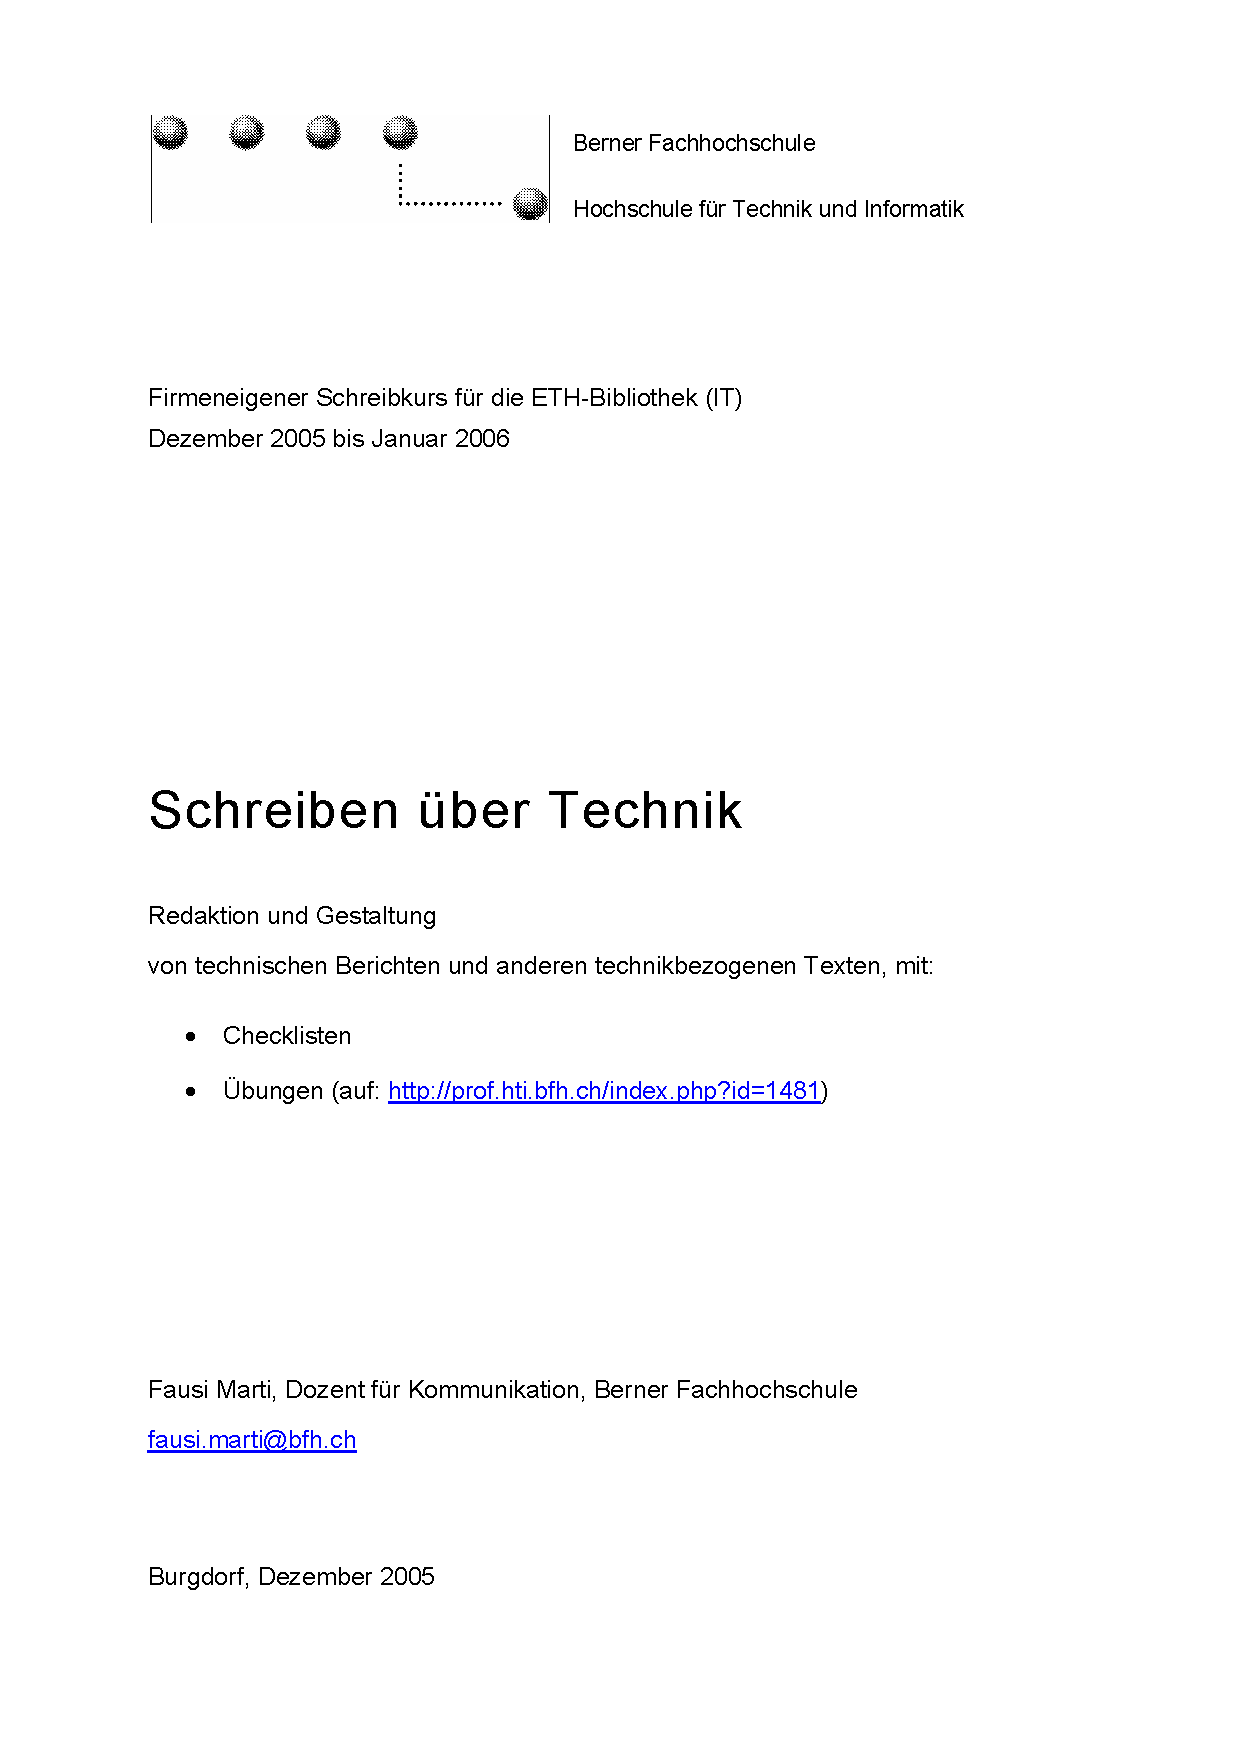
\includepdf[scale=0.7,pagecommand={},page=-,landscape=false]{appendix/technischer_bericht/src/techschreiben.pdf}
  
%
%
%
\end{document}
